%!TEX root = ../thesis.tex

\chapter{Preliminaries}
\label{chap:prelim}
\section{Setting}
\subsection{Classification} 
\label{subsec:class}
We will now provide a formal description of the settings used in this thesis. The first setting is that of \textit{classification}\cite{Hastie2009}. In this setting we are presented with training examples and their correct label. We must then study these examples and come up with a rule to classify future unlabelled inputs. Here we have a finite amount of labels lacking any structure like order or magnitude. We will primarily concern ourselves with binary classification, i.e. results being either negative or positive, since the generalization to multi-class problems has been studied in \cite{Freund1997} and is outside the scope of this thesis. An example of this setting is spam detection. Given enough example emails labelled correctly, we must formulate a rule to label new incoming emails as either genuine or spam. 
\par In this setting we have an input and a label space, denoted $\mathcal X$ and $\mathcal Y$ respectively. For the remainder of this thesis we will generally set $\mathcal X = \R^d$ and $\mathcal Y = \set{0,1}$ or $\mathcal Y = \set{-1,1}$, the later choice depending on convenience. We will differentiate between generic, or hypothetical, and actually observed data by denoting the former with upper case  and the later by lower case letters. Furthermore vectors will be denoted in boldface and their components will be denoted by a subscript $k$. We will denote out data as follows: $\Vec{Y_1\\ \mathbf X_1},\ldots, \Vec{Y_i\\ \mathbf X_i},\ldots,\Vec{Y_N\\ \mathbf X_N}$, where $i$ is the $i$th example ranging from 1 to $N$. So to summarize: $X_{i,k}$ is the $k$th component of the $i$th generic example $\mathbf X_i$. Generally any operation written using vectors, which may or may not be formally defined, is used to mean component wise operations.  Finally since all algorithms are iterative we will use a superscript $t$ to denote instances at time (or iteration) $t$, so if we for example have a distribution $\vec p$ then $\vec p^t$ is the distribution on the $t$th iteration, with components $ p^t_k$ where $t$ will generally range from $1$ to $T$ and $k$ from 1 to $d$

\subsection{Hedging}
\label{subsec:hedging}
In the context of hedging we will have to allocate our resources according to several strategies, in such a way that we minimize our losses. An example of this process would be the following: imagine you are betting on a horse race. You have several friends all of whom advise you according to some rule of thumb and you want to bet a fixed amount on every round. If you knew ahead of time which rule of thumb would be the best you would bet everything according to that rule, but this is usually not known. You try do distribute your betting money in such a way that your losses won't be much worse than if you bet everything according to your luckiest friend. 
\par Formally this means that an agent $A$ has access to $N$, \textit{strategies}, often also called \textit{experts}, will attempt to choose a distribution $\vec p^t$ over these strategies at every round, for $T$ rounds. After choosing $\vec p^t$ we will receive a loss vector which we will denote as $\Bell^t$, and suffer loss equal to $$\sum_{i=1}^N p^t_i\ell_i^t = \vec p^t \cdot \Bell^t.$$ In this context we will denote the loss of the $i$th strategy as $$L_i:= \sum_{t=1}^T \ell^t_i$$ and the loss of $A$ as $$L_A := \sum_{t=1}^T \vec p^t \cdot \Bell^t.$$ Our goal is to minimize what is called the \textit{regret} which is defined as $$R_A:=L_A - \min_i L_i$$ i.e. the difference in the suffered loss and the minimal loss we could have had. 

\subsection{Weak learners}
\label{subsec:weak}
In the context of boosting we will often require algorithms which are called \textit{weak probably approximately correct(PAC) learning algorithms}\cite{Freund1997}, to which we will refer as \textit{weak learners}. We will furthermore use $\weak$ to denote a generic weak learning algorithm. These weak learners must satisfy the following conditions: given some $\delta,\gamma >0$ and access to enough examples this algorithm must output an hypothesis that has training error at most $\ve \leq \frac12 - \gamma$ with probability $1-\delta$. This means that the algorithm must, with a certain probablity (the P in PAC), provide an hypothesis that performs at least slightly better than random guessing(the AC in PAC) on the training set. This low training error will then be expected to generalize to a hopefully low generalization error. The generalization error refers to the error on a set of examples that also has their correct labels attached but was not used to train the algorithm but to test it after the training is done. This is to avoid something called \textit{over fitting} and refers to the phenomenon that the rules constructed by the algorithms are overly complicated, which leads to the algorithm performing very well on the training data but not on new data. 

\par In this thesis the role of the weak learners will mostly be fulfilled by what are called \textit{decision stumps}. These are decision trees of depth one i.e. the learner will measure a single feature of an input and then attempt to formulate an answer. Formally this means that given an input $\vec X$ the stump will attempt to find an optimal $r$ and $k$ such that  the hypothesis $h:\mathcal X \to \mathcal Y$ given by $$h(\mathbf X):= \begin{cases}1 &\text{if } X_k \leq r\\-1&\text{otherwise}\end{cases}$$ has minimal error on our training set. Here we have chosen to check whether $X_k\leq r$ instead of  $X_k\geq r$ but this is another choice for which the stump can optimize. 

\subsection{Boosting}
\label{subsec:boosting}
The setting of boosting is as follows: we require a set of correctly labeled training data and a weak learning algorithm $\weak$. Often a boosting algorithm can also accept a distribution on the training data to exploit any prior knowledge one might have, which is set to the uniform distribution if no extra knowledge is provided. The procedure is at each iteration is to fit \weak on the training data which provides us with an hypothesis $h^t:\mathcal X \to \mathcal Y$. Using this hypothesis we will calculate a loss vector $\Bell^t$. This loss vector is a measure for how well $\weak$ performed on the training data and is usually some form of the training error. For example $\adaB$ uses the weighted error $\vec p^t\cdot\Bell^t$ whereas \NHB also uses a measure called the margin and its distribution, which we will define in section \ref{subsec:NHAlgo}. Using this loss vector we will slightly alter the training set by attaching weights to them, which measure their relative importance and then repeat the process. Our final hypothesis will then be some weighted majority vote among all of the hypotheses. 

\newpage
\section{AdaBoost}
\label{sec:ada}

\begin{algorithm} 
\caption{\adaB}
\label{fig:adaCode}
	\begin{algorithmic}[1]
	\Require 
	\Statex $N$ labelled samples $\Vec{y_1\\ \mathbf x_1},\ldots,\Vec{y_N\\ \mathbf x_N}$  with $\mathcal Y = \set{0,1}$ 
	\Statex Distribution $D$ over the $N$ examples
	\Statex Weak learning algorithm $\weak$
	\Statex Number of trials $T$
	\Procedure{\textbf{AdaBoost}}{}
	\State \textbf{Initialize} the weight vector $w_i^1=D(i)$ for $i=1,\ldots,N$
	\For {$t= 1,2,\ldots,T$}
	\State Set $$\bf p^t= \frac{\bf w^t}{\sum_{i=1}^N w^t_i}$$
	\State Call \weak($\bf p^t$) and receive hypothesis $h^t:\mathcal X\to\mathcal Y$
	\State Calculate the error of $h^t:\ve^t=\sum^N_{i=0}p^t_i|h^t(\mathbf x_i)-y_i|$
	\State Set $\b_t=\ve^t/(1-\ve^t)$
	\State Update the weights $$w_i^{t+1}=w_i^t\beta^{1-|h^t(\vec x_i)-y_i|}_t$$
	\EndFor\\
	\Return $$h_f(\mathbf x)=\begin{cases}1 & \text{if } \sum^T_{t=0}(\log1/\b_t)h^t(\mathbf x)\geq\frac12\sum^T_{t=0}\log1/\b_t\\0&\text{otherwise}\end{cases}$$
	\EndProcedure
	\end{algorithmic}
\end{algorithm}
\subsection{The algorithm}
\label{subsec:AdaAlgo}
We will now give a formal discussion of the \adaB\cite{Freund1997} algorithm, which can be found in algorithm \ref{fig:adaCode} above. The goal of the algorithm is to minimize the error with the respect to the distribution 
%\todo[line]{vind een betere notatie voor initial distribution} 
over the training data. In the first step the learner will obtain a new distribution by normalizing the weights from the previous step, or from the initial distribution. This distribution will then be provided to \weak which will form a hypothesis accordingly. When the hypothesis is formulated the learner will calculate it's error and set the parameter $\beta$, which can be interpreted as the learning speed. In the final step the learner will update the weights appropriately. It is important to observe that \weak produces an hypothesis at every iteration and that the final hypothesis is essentially a weighted majority vote among all of these hypotheses. 

\subsection{The theoretical performance of \adaB}
\label{subsec:AdaTheoPerf}
Here we will discuss the theoretical performance of \adaB. One of the main results from \cite{Freund1997}, is the following theorem: 
\begin{theorem}\label{thm:adaErr}\cite{Freund1997}
Suppose \adaB runs for $T$ rounds calling the weak learning algorithm \weak which generates hypotheses with errors $\ve_1\ldots, \ve_T$ (as defined in step 3 in algorithm \ref{fig:adaCode}). Then the error $\ve:=\Pr_{i\sim D}[h_f(x_i)\neq y_i]$ of the final hypothesis $h_f$ output by \adaB is bounded above by $$\ve\leq 2^T\prod^T_{t=1}\sqrt{\ve_t(1-\ve_t)}$$
\end{theorem}
We will omit the proof since it is not the focus of this thesis but we will briefly discuss its consequences. As discussed above one might find it strange that every hypothesis is allowed a vote in the final hypothesis. This is still, however, an improvement over previous algorithms since the final error will now depend on the error of all hypotheses instead of only the worst, as was the case in previous works. It is also not immediately obvious that this upper bound does us any good since it contains exponents and products for which it is not trivial how they cancel out. In their paper Freund and Shapire reduce the above stated upper bound to the following one: $$\ve\leq \exp\left(-2\sum^T_{t=0}\gamma_t^2\right)$$ where the $\gamma_t$ is defined such that $\ve_t=1/2-\gamma_t$ holds. This upper bound is more useful since it decreases exponentially, leading us to conclude that \adaB has a good theoretical performance.   

\subsection{The practical performance of \adaB}
\label{subsec:AdaPracPerf}
In an attempt to demonstrate the practical performance we recreated the following situation from \cite{Hastie2009}. We have ten features $X_1,\ldots,X_{10}$ which are drawn from a standard independent Gaussian. Their label is determined (deterministically) by the following rule: $$Y:=\begin{cases}
1 & \sum_{i=0}^{10} X^2_i > \chi_{10}^2(0.5)\\
0 & \text{otherwise}
\end{cases}$$ Where $\chi_{10}^2(0.5)=9.34$ is the median of a chi-squared random variable with ten degrees of freedom. The results of testing can be found in figure \ref{fig:adaB} and will be discussed below. 

\begin{figure}[!ht]
  \centering
      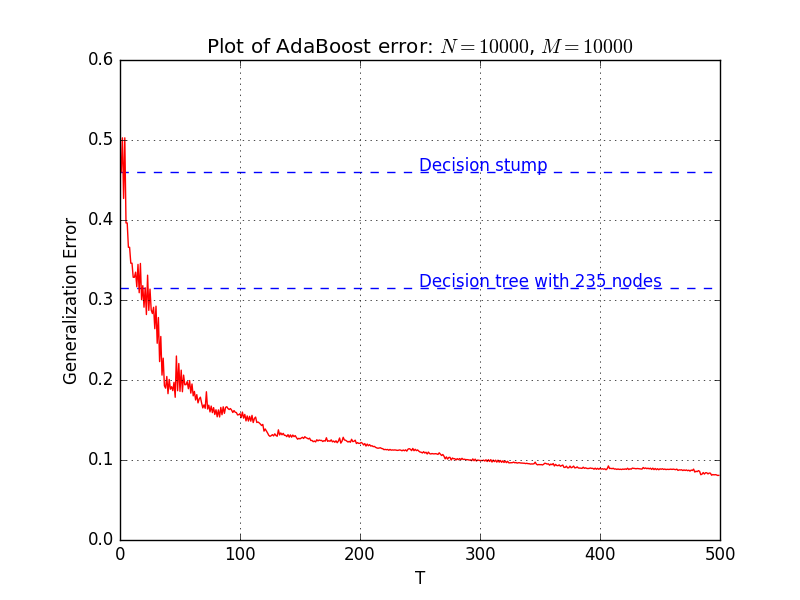
\includegraphics[width=0.8\textwidth]{generated/prettyLong.png}
  \caption{Generalization error of AdaBoost as a function of number of iterations with 10000 examples and test cases. The error of actual stumps and a tree with 217 nodes is also shown for reference}
      \label{fig:adaB}
\end{figure}

First of all it should be noted that we took an equal amount of training and testing examples (10000 to be exact). This is was possible because we can generate the data ourselves in a reasonable amount of time. In practical settings this is however usually not the case and one would need to reserve a portion of their data for testing instead of training. This means that the more testing one does, the less training one can do an thus, generally one would reserve only around 10\% of their data for testing.
\par Looking at figure \ref{fig:adaB} it is obvious that our algorithm works. The decision stump initially performs with an error rate of 47\% which is indeed only just better than random guessing. \adaB outperforms this and even a large tree with 217 nodes and an error rate of 30\% after just tenths of iterations and reaches an error rate as low as 8\% after 400 iterations. 

\section{\NHB}
\label{sec:NHB}
\subsection{The algorithm}
\label{subsec:NHAlgo}
In their paper \cite{Luo2014} Luo and Schapire use the framework they had previously developed for drifting game analysis to develop a new algorithm called \adaN which improves upon the previous \textbf{NormalHedge} algorithm. Whereas \textbf{NormalHedge} depends on a numerical search to find the right parameters Luo and Schapire first develop a general setting for Hedge algorithms which requires convex functions as input and then proceed to derive a parameter free version which they called \adaN. This algorithm was much more computationally efficient and was easier to generalize to other settings such as boosting. They then proceeded to indeed generalize this to several settings including boosting, which lead them to derive the \NHB algorithm which we will discuss here. 
\begin{algorithm} 
\caption{\NHB}
\label{fig:adaNCode}
\begin{algorithmic}[1]
\Require 
\Statex $N$ labelled samples $\Vec{y_1\\ \mathbf x_1},\ldots,\Vec{y_N\\ \mathbf x_N}$  with $\mathcal Y = \set{-1,+1}$ 
\Statex Weak learning algorithm $\weak$
\Statex Number of trials $T$
\Procedure{\adaN}{}
\State \textbf{Initialize} $\mathbf{s}_0 = \mathbf 0$
\For {$t= 1,2,\ldots,T$}
\State Set: $\mathbf p^t \propto \exp([\mathbf s^{t-1}-1]_-^2/3t) - \exp([\mathbf s^{t-1}+1]_-^2/3t) $ 
\State Call $\weak(\mathbf p^t)$ and get hypothesis $h^t$ with edge $\gamma^t = \frac12\sum_{i=1}^Np^t_iy_ih^t(\mathbf x_i)$
\State Set: $\mathbf s^t = \mathbf s^{t-1} + \frac12 y_ih^t(\mathbf x_i)-\gamma^t$
\EndFor\\
\Return $H(\mathbf x) = \sign\lubke{\sum^T_{t=1}h^t(\mathbf{x})}$
\EndProcedure
\end{algorithmic}
\end{algorithm}

\subsection{The theoretical performance of \NHB}
\label{subsec:NHTheoPerf}
Again \NHB uses several instances of \weak, which are all expected to have \textit{edge} at least $\gamma$, i.e. have error $\frac12 - \gamma$ w.r.t. the training distribution, to form a comity which decides a final output based on a majority vote. In their paper they formulate and proved the following theorem: 
 \begin{theorem}\label{Thm:NHBPerf}\cite{Luo2014}
 After $T$ rounds the training error of \NHB is of order $\mathcal{O}(\exp(-\frac13T\gamma^2))$ and the fraction of training example with margin at most $\theta(\leq2\gamma)$ is of order $\mathcal{O}(\exp(-\frac13T(\theta-2\gamma)^2))$

 \end{theorem}

 We will again omit the proof but briefly discuss its consequences here. Firstly it is useful to observe that the training error of \NHB is comparable to that of \adaB. However instead of looking just at the training error and trying to generalize that to the generalization error Luo and Schapiere also make statements with respect to the margin distribution which is a measure of confidence often used in regression settings. The margin of a example with respect to some weak learner is defined as $\frac1T \sum^T_{t=1}yh^t(x)$ i.e. the difference between the fractions of correct and incorrect hypothesis on the example respectively. Here it's magnitude measures the confidence of the committee and it's sign measures whether the weak learner was correct or not. In this light the above theorem also states that the fraction of training examples the algorithm deems important enough also decreases exponentially and thus it ignores a lot of examples every round, making it much more computationally efficient. 

 \subsection{The practical performance of \NHB}
 \label{subsec:NHPracPerf}
